\chapter{La gravitation}\label{ch:g9:gravitation}

Une pomme lâche sa branche et tombe. La \omterm{def:g2:moon-in-the-sky:moon}{Lune}, au-dessus du même
verger, ne tombe pas. Pendant des milliers d'années, cela sembla deux
faits sans rapport --- jusqu'à ce qu'une intuition de génie les
réunisse~: la \omterm{def:g2:moon-in-the-sky:moon}{Lune} \emph{est} en train de tomber, sans fin, autour de
la Terre, retenue par l'attraction même qui réclame la pomme. Une
seule loi pour le verger et pour le ciel --- l'équation la plus
audacieuse jamais écrite à ce jour, et ta dernière année de ce livre
s'ouvre sur elle.

\section{L'attraction universelle}

\begin{definition}[Gravitation]\label{def:g9:gravitation:gravitation}
La \emph{gravitation}\index{gravitation} est l'attraction mutuelle
entre toutes les \omterm{def:g3:measuring-mass:mass}{masses}~: chaque portion de matière de l'Univers
\omterm{def:g1:magnets:magnet}{attire} toutes les autres. C'est la \omterm{def:g2:pushes-and-pulls:force}{force} sans contact que tu as
rencontrée sous le nom d'«~attraction de la Terre~» il y a des années
--- révélée maintenant comme universelle~: la Terre \omterm{def:g1:magnets:magnet}{attire} la pomme,
la pomme \omterm{def:g1:magnets:magnet}{attire} la Terre, la \omterm{def:g2:moon-in-the-sky:moon}{Lune} \omterm{def:g1:magnets:magnet}{attire} les mers, le Soleil \omterm{def:g1:magnets:magnet}{attire}
les \omterm{def:g4:solar-system:planet}{planètes}, et deux livres sur une étagère s'attirent l'un l'autre,
faiblement, pour toujours.
\end{definition}

\begin{proposition}[La loi de la gravitation universelle]\label{prop:g9:gravitation:law}
Deux corps de \omterm{def:g3:measuring-mass:mass}{masses} $m_A$ et $m_B$ (en \unit{kg}), dont les centres
sont distants de $d$ (en \unit{m}), s'attirent l'un l'autre par des
\omterm{def:g2:pushes-and-pulls:force}{forces} égales et opposées, portées par la droite qui les joint, et de
valeur
\[
F = G \times \frac{m_A \times m_B}{d^2},
\]
$F$ en newtons (\unit{N}) --- l'\omterm{def:g6:measurement-in-science:measuring}{unité} de \omterm{def:g2:pushes-and-pulls:force}{force} dont l'histoire
complète commence au chapitre suivant --- avec
$G = \qty{6.67e-11}{N.m^2/kg^2}$, la \emph{constante
gravitationnelle}, le même nombre partout dans l'Univers. La \omterm{def:g2:pushes-and-pulls:force}{force}
croît avec chacune des \omterm{def:g3:measuring-mass:mass}{masses}, et meurt avec le \emph{carré} de la
distance~: deux fois plus loin, quatre fois plus faible~; dix fois
plus loin, cent fois plus faible.
\end{proposition}

\begin{omfigure}
\begin{tikzpicture}[scale=0.85]
  \draw[thick, fill=omDef, fill opacity=0.4] (1.4,1.4) circle (0.65);
  \node[font=\small] at (1.4,1.4) {$m_A$};
  \draw[thick, fill=omThm, fill opacity=0.4] (8.6,1.4) circle (0.45);
  \node[font=\small] at (8.6,1.4) {$m_B$};
  \draw[-Stealth, very thick, omThm] (2.15,1.4) -- (3.55,1.4);
  \draw[-Stealth, very thick, omDef] (8.05,1.4) -- (6.65,1.4);
  \draw[Stealth-Stealth, omExo] (1.4,0.45) -- (8.6,0.45);
  \node[below, font=\small, omExo] at (5.0,0.35) {$d$};
  \node[above, font=\small] at (5.0,1.75)
    {attractions égales, sens opposés --- toujours les deux};
\end{tikzpicture}

{\small La \omterm{def:g9:gravitation:gravitation}{gravitation} universelle~: deux \omterm{def:g3:measuring-mass:mass}{masses}, deux attractions
égales et opposées le long de la droite qui les joint --- la pomme
\omterm{def:g1:magnets:magnet}{attire} la Terre exactement aussi fort que la Terre \omterm{def:g1:magnets:magnet}{attire} la pomme.}
\end{omfigure}

\begin{example}[Lire la loi]\label{ex:g9:gravitation:reading}
Chaque trait de la formule parle. Les \omterm{def:g3:measuring-mass:mass}{masses} se multiplient~: double
l'un ou l'autre partenaire, tu doubles la \omterm{def:g2:pushes-and-pulls:force}{force}. La distance est au
carré au dénominateur~: la \omterm{def:g9:gravitation:gravitation}{gravitation} est un murmure qui s'éteint
vite --- la dilution en carré inverse que tu retrouveras avec la
\omterm{def:g1:light-and-shadows:source}{lumière} et le \omterm{def:g3:sound-around-us:sound}{son}, car c'est la géométrie de tout ce qui se répand
dans l'espace. Et la taille minuscule de $G$ --- onze zéros après la
virgule --- proclame la \omterm{def:g9:gravitation:gravitation}{gravitation} le \omterm{def:g4:weight-and-mass:weight}{poids} plume des \omterm{def:g2:pushes-and-pulls:force}{forces} de la
nature~: elle ne règne sur le cosmos que parce que les \omterm{def:g3:measuring-mass:mass}{masses} de
là-haut sont monstrueuses et que rien ne la compense.
\end{example}

\begin{example}[Pourquoi les étagères ne se referment pas d'un coup]\label{ex:g9:gravitation:books}
Deux livres de \qty{1}{kg}, centres distants de \qty{0.1}{m}~:
\[
F = \num{6.67e-11} \times \frac{1 \times 1}{0.1^2}
= \qty{6.67e-9}{N}
\]
--- quelques milliardièmes de newton, autant dire le \omterm{def:g4:weight-and-mass:weight}{poids} d'une
poussière de poussière. Maintenant la Terre et la pomme~: remplace
un livre par \qty{5.97e24}{kg} de \omterm{def:g4:solar-system:planet}{planète} et la distance par son
rayon de \qty{6.4e6}{m}, et la même loi livre la traction familière
d'un après-midi au verger. Universel veut dire universel --- seules
les \omterm{def:g3:measuring-mass:mass}{masses} décident de qui s'en aperçoit.
\end{example}

\section{La Lune qui tombe}

\begin{example}[Le canon sur la montagne]\label{ex:g9:gravitation:cannon}
L'expérience de pensée de l'intuition elle-même. Tire un boulet de
canon à l'horizontale depuis un haut sommet~: il décrit un arc et
retombe. Tire-le plus vite~: il retombe plus loin --- l'attraction de
la Terre courbant sa \omterm{def:g6:describing-motion:trajectory}{trajectoire} tout du long. Imagine maintenant de
le tirer si vite que, pendant qu'il tombe, la surface de la Terre
ronde \emph{s'écarte sous lui à la même allure}~: le boulet tombe sans
fin et ne retombe jamais --- il fait le tour de la \omterm{def:g4:solar-system:planet}{planète}. Cette
chute perpétuelle porte un nom familier~: une \emph{\omterm{def:g6:sun-earth-moon:axisorbit}{orbite}}. Rien ne
tient «~en l'\omterm{def:g2:air-around-us:air}{air}~» un corps en \omterm{def:g6:sun-earth-moon:axisorbit}{orbite}~; il tombe avec panache.
\end{example}

\begin{omfigure}
\begin{tikzpicture}[scale=0.85]
  % the curving Earth: only the upper limb of a much larger circle
  \fill[omDef, opacity=0.25] (-1.01,0.23) arc (106:74:20)
    -- (10.01,-0.9) -- (-1.01,-0.9) -- cycle;
  \draw[thick] (-1.01,0.23) arc (106:74:20);
  % the mountain and its gun
  \draw[thick, fill=omExo!30]
    (-1.1,0.2) -- (0.25,2.3) -- (1.3,0.72) -- cycle;
  \draw[thick, fill=omExo!60] (0.0,2.18) rectangle (0.55,2.42);
  \node[left, font=\small] at (-0.85,2.3) {le canon du sommet};
  % three shots, each faster than the last
  \draw[omThm, thick] (0.55,2.32)
    .. controls (1.6,2.25) .. (2.4,0.9);
  \draw[omThm, thick] (0.55,2.35)
    .. controls (2.8,2.25) .. (4.9,1.0);
  \draw[omThm, thick] (0.55,2.38)
    .. controls (4.2,2.35) .. (7.5,0.8);
  \node[right, font=\small, omThm] at (1.9,3.0)
    {plus vite~: plus loin};
  % fast enough: the fall closes into an orbit
  \draw[omMeth, very thick, dashed] (0.3,2.35) arc (101:73:21.76);
  \node[right, font=\small, omMeth] at (6.4,3.35)
    {assez vite~: la chute devient orbite};
\end{tikzpicture}

{\small Le canon de la montagne~: chaque tir plus rapide tombe plus
loin autour de la Terre qui se courbe --- jusqu'à ce que la chute et
la courbure s'accordent, et que le boulet se mette en \omterm{def:g6:sun-earth-moon:axisorbit}{orbite}.}
\end{omfigure}

\begin{proposition}[Ce que fait tourner la gravitation]\label{prop:g9:gravitation:runs}
Une seule loi, tout le ciel~: la \omterm{def:g2:moon-in-the-sky:moon}{Lune} est l'éternel boulet de canon de
la Terre, qui tombe autour de nous une fois par mois~; les \omterm{def:g4:solar-system:planet}{planètes}
tombent de même autour du Soleil --- les plus proches plus vite, comme
l'exige le carré inverse~; les comètes plongent depuis le noir sur de
longues boucles de chute~; et tout satellite artificiel --- yeux
météorologiques, balises de navigation, station habitée qui tourne
toutes les quatre-vingt-dix minutes --- roule sur les mathématiques du
canon de la montagne. Rien n'est suspendu dans les cieux. Tout tombe,
et tout manque sa cible.
\end{proposition}

\begin{example}[Les marées~: la Lune attire en retour]\label{ex:g9:gravitation:tides}
La mutualité a une signature écrite dans l'eau. L'attraction de la
\omterm{def:g2:moon-in-the-sky:moon}{Lune} sur la Terre est la plus forte sur l'océan qui lui fait face et
la plus faible de l'autre côté --- si bien que les mers se soulèvent
doucement vers la \omterm{def:g2:moon-in-the-sky:moon}{Lune} et à l'opposé de la \omterm{def:g2:moon-in-the-sky:moon}{Lune} à la fois~; et comme
la Terre tourne sous ces bourrelets, les côtes voient l'eau monter et
descendre~: les \emph{marées}, deux fois par jour la plupart du temps.
Le Soleil y met la main --- aligné à la nouvelle et à la \omterm{ex:g2:moon-in-the-sky:shapes}{pleine lune}
pour les grandes marées de vives-eaux. Les pêcheurs lisent la \omterm{def:g2:moon-in-the-sky:moon}{Lune}
depuis des millénaires~; la loi la leur relit.
\end{example}

\begin{remark}[Ce que la loi ne dit pas]\label{rem:g9:gravitation:notsay}
La grande équation calcule la \omterm{def:g2:pushes-and-pulls:force}{force} avec une exactitude exquise et
n'explique pas d'un iota \emph{comment} deux corps se saisissent à
travers le vide --- son auteur lui-même déclara la question ouverte et
la laissa, magnifiquement, sans réponse. Des réponses plus profondes
existent --- les années d'université de ce cours atteignent la
réponse moderne, où la \omterm{def:g3:measuring-mass:mass}{masse} courbe la géométrie même qu'elle habite
--- mais tout physicien honnête depuis lors a répété la leçon que tu
peux tirer de cette page~: une loi peut être parfaitement utile,
parfaitement éprouvée, et garder pourtant son ultime secret.
\end{remark}

\begin{omfigure}
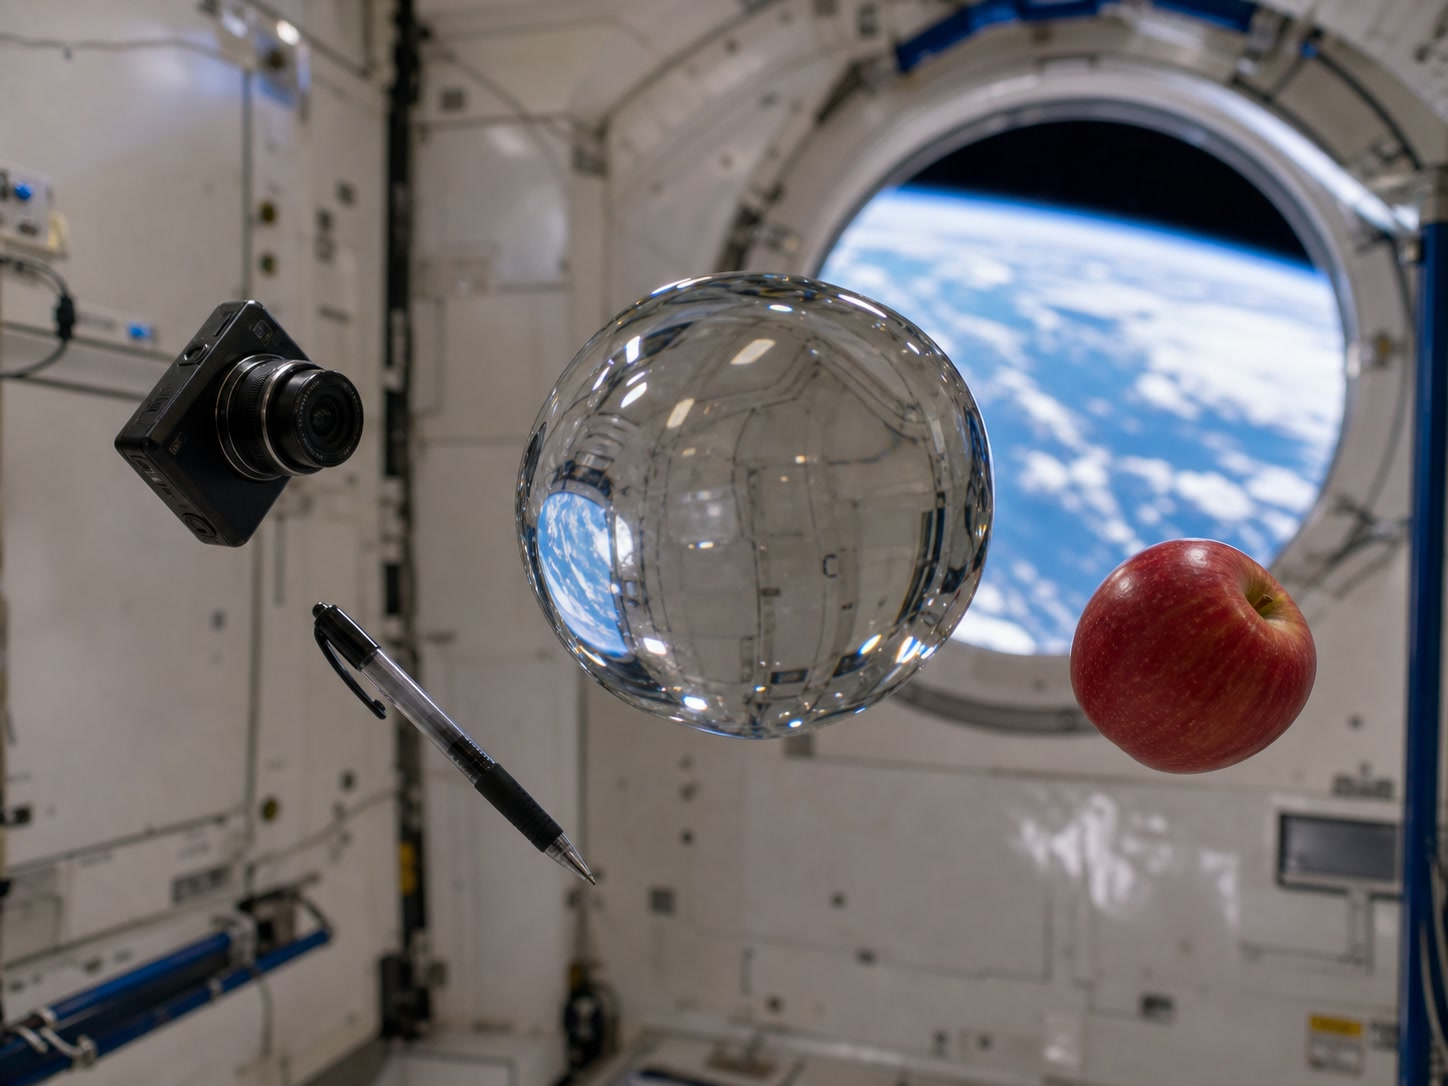
\includegraphics[width=0.5\linewidth]{images/book1/ai/g9-gravitation-weightless.jpg}

{\small La chute libre, vécue tous les jours~: la station spatiale et tout ce qu'elle contient tombent ensemble autour de la Terre, si bien que rien n'appuie sur rien --- appareils photo, stylos, pommes et eau flottent.}
\end{omfigure}

\section{Exercices}

\begin{exercise}[$\star$]\label{exo:g9:gravitation:1}
Énonce la loi de la \omterm{def:g9:gravitation:gravitation}{gravitation} universelle --- formule, \omterm{def:g6:measurement-in-science:measuring}{unités}, et
les deux traits (les \omterm{def:g3:measuring-mass:mass}{masses}, la distance) avec des mots.
\end{exercise}

\begin{exercise}[$\star$]\label{exo:g9:gravitation:2}
La Terre \omterm{def:g1:magnets:magnet}{attire} la pomme avec \qty{1}{N}. Avec quelle \omterm{def:g2:pushes-and-pulls:force}{force} la pomme
attire-t-elle la Terre~? Pourquoi une seule des deux
accélère-t-elle visiblement~?
\end{exercise}

\begin{exercise}[$\star$]\label{exo:g9:gravitation:3}
Deux satellites sont en \omterm{def:g6:sun-earth-moon:axisorbit}{orbite} à des distances $d$ et $2d$ du centre
de la Terre. Compare les \omterm{def:g2:pushes-and-pulls:force}{forces} gravitationnelles qu'ils subissent
(\omterm{def:g3:measuring-mass:mass}{masses} égales). Et à $10 d$~?
\end{exercise}

\begin{exercise}[$\star$]\label{exo:g9:gravitation:4}
Calcule l'attraction entre deux danseurs de \qty{80}{kg} distants de
\qty{0.5}{m} --- et commente le romantisme au regard de la
\omterm{def:g9:gravitation:gravitation}{gravitation}.
\end{exercise}

\begin{exercise}[$\star$]\label{exo:g9:gravitation:5}
Dans l'histoire du canon de la montagne, quelles deux allures
s'accordent exactement pour le tir mis en \omterm{def:g6:sun-earth-moon:axisorbit}{orbite}~? Qu'est-ce qu'une
\omterm{def:g6:sun-earth-moon:axisorbit}{orbite}, en trois mots~?
\end{exercise}

\begin{exercise}[$\star$]\label{exo:g9:gravitation:6}
«~Les astronautes flottent parce qu'il n'y a pas de gravité là-haut.~»
Démolis cela avec le boulet de canon~: que font, l'une et l'autre, la
station et son équipage~?
\end{exercise}

\begin{exercise}[$\star$]\label{exo:g9:gravitation:7}
Pourquoi la \omterm{def:g9:gravitation:gravitation}{gravitation}, \omterm{def:g4:weight-and-mass:weight}{poids} plume de la nature, gouverne-t-elle
malgré tout le cosmos~? Deux raisons tirées du chapitre.
\end{exercise}

\begin{exercise}[$\star$]\label{exo:g9:gravitation:8}
D'où viennent les marées, et pourquoi deux fois par jour la plupart du
temps~? Quand les plus grandes frappent-elles~?
\end{exercise}

\begin{exercise}[$\star\star$]\label{exo:g9:gravitation:9}
La \omterm{def:g2:moon-in-the-sky:moon}{Lune} (\qty{7.3e22}{kg}) est en \omterm{def:g6:sun-earth-moon:axisorbit}{orbite} à \qty{3.8e8}{m} de la Terre
(\qty{5.97e24}{kg}). Calcule leur attraction, en notation
scientifique du début à la fin --- et admire le nombre de chiffres que
porte la puissance de dix du résultat.
\end{exercise}

\begin{exercise}[$\star\star$]\label{exo:g9:gravitation:10}
À la surface de la \omterm{def:g2:moon-in-the-sky:moon}{Lune}, ton \omterm{def:g4:weight-and-mass:weight}{poids} se réduisait au sixième
(souviens-toi des astronautes qui bondissaient). En te servant des
deux réglages de la loi --- la \omterm{def:g3:measuring-mass:mass}{masse} plus petite de la \omterm{def:g2:moon-in-the-sky:moon}{Lune}, son rayon
plus petit --- explique comment un sixième peut sortir d'un corps
quatre-vingts fois plus léger que la Terre.
\end{exercise}

\begin{exercise}[$\star\star$]\label{exo:g9:gravitation:11}
Mercure boucle son tour du Soleil en $88$ jours, Neptune en $165$ ans.
Lis ce motif dans le carré inverse~: que fait l'affaiblissement de la
\omterm{def:g9:gravitation:gravitation}{gravitation} avec la distance à la poigne du Soleil, et donc à l'allure
de la famille extérieure~?
\end{exercise}

\begin{exercise}[$\star\star\star$]\label{exo:g9:gravitation:12}
Un satellite géostationnaire se tient apparemment immobile au-dessus
d'un point de l'équateur --- les antennes paraboliques ne bougent
jamais. Concilie cette apparence avec
\cref{prop:g9:gravitation:runs}~: que doit valoir sa période
orbitale, dans quel sens doit-il tourner, et pourquoi «~se tenir~» ici
veut-il dire «~tomber au pas parfait de la Terre qui tourne~»~?
\end{exercise}

\section{Problème~: l'héritage du boulet de canon}

\begin{problem}[{Problème du week-end --- du verger à l'orbite~; la
pomme, le canon et la Lune audités avec une seule loi~; le tableau des
lancements}]\label{pb:g9:gravitation:1}
Une soirée au pupitre de vulgarisation de l'agence spatiale~: une
seule loi, $G = \qty{6.67e-11}{N.m^2/kg^2}$, \omterm{def:g3:measuring-mass:mass}{masse} de la Terre
\qty{5.97e24}{kg}, rayon de la Terre \qty{6.4e6}{m}.

\medskip\noindent\textbf{Partie I --- l'audit de la pomme.}
\begin{enumerate}
  \item Calcule l'attraction de la Terre sur une pomme de
        \qty{0.1}{kg} à la surface (centres séparés d'un rayon
        terrestre).
  \item Avec quelle \omterm{def:g2:pushes-and-pulls:force}{force} la pomme attire-t-elle la Terre en
        retour~? Donne le mot de la loi pour cette comptabilité à
        double sens.
  \item Élève la pomme jusqu'à deux rayons terrestres du centre.
        Que devient l'attraction~?
  \item Un visiteur demande pourquoi la formule emploie la distance
        au \emph{centre} de la Terre plutôt qu'au sol. Offre la
        réponse courte et honnête (la \omterm{def:g4:solar-system:planet}{planète} entière \omterm{def:g1:magnets:magnet}{attire}, et
        ses attractions dispersées s'additionnent comme si elles
        venaient du centre --- un théorème que le grand auteur
        lui-même mit des années à démontrer).
\end{enumerate}

\medskip\noindent\textbf{Partie II --- le tableau des lancements.}
\begin{enumerate}[resume]
  \item Le satellite du jour a une \omterm{def:g3:measuring-mass:mass}{masse} de \qty{2000}{kg}. Son
        \omterm{def:g4:weight-and-mass:weight}{poids} à la surface, par la loi~? (Ou par le raccourci que
        nomme le chapitre suivant~: environ \qty{9.8}{N} par
        \omterm{def:g3:measuring-mass:units}{kilogramme}.)
  \item Sur son \omterm{def:g6:sun-earth-moon:axisorbit}{orbite} de travail, à \qty{1.28e7}{m} du centre ---
        deux rayons terrestres --- quelle fraction de son \omterm{def:g4:weight-and-mass:weight}{poids} de
        surface la \omterm{def:g9:gravitation:gravitation}{gravitation} exerce-t-elle encore sur lui~?
  \item «~Il y a donc encore une vraie gravité là-haut~?~»
        Confirme avec le nombre --- et explique ce que le satellite
        fait de cette attraction au lieu de s'écraser.
  \item Le commentaire du lancement dit que «~la \omterm{def:g7:motion-average-speed:formula}{vitesse} orbitale
        doit s'accorder à la chute~». Raconte de nouveau l'histoire
        du canon de la montagne en deux phrases pour la brochure
        des visiteurs.
\end{enumerate}

\medskip\noindent\textbf{Partie III --- le grand livre de la \omterm{def:g2:moon-in-the-sky:moon}{Lune}.}
\begin{enumerate}[resume]
  \item La \omterm{def:g2:moon-in-the-sky:moon}{Lune} étant à \qty{3.8e8}{m}, à combien de rayons
        terrestres roule-t-elle~? (Une décimale.)
  \item Par le carré inverse, la \omterm{def:g9:gravitation:gravitation}{gravitation} là-bas s'est
        affaiblie jusqu'à environ quelle fraction de sa valeur en
        surface~? (Élève au carré ta réponse précédente.)
  \item La grande intuition, redite~: la pomme du verger tombe
        d'environ cinq \omterm{def:g2:measuring-length:units}{mètres} dans sa première seconde~; la \omterm{def:g2:moon-in-the-sky:moon}{Lune},
        chaque seconde, «~tombe~» vers la Terre d'à peine un
        millimètre --- et n'arrive pourtant jamais. Relie les deux
        faits par tes réponses 9 et 10~: pourquoi la chute de la
        \omterm{def:g2:moon-in-the-sky:moon}{Lune} est-elle des milliers de fois plus douce, et pourquoi
        est-elle sans fin~?
  \item Clos la soirée de vulgarisation~: une loi, trois
        interprètes --- la pomme, le satellite, la \omterm{def:g2:moon-in-the-sky:moon}{Lune}. Écris la
        phrase de conclusion du pupitre qui les réunit.
\end{enumerate}
\end{problem}
